%% CorpusSLR - SoftwareX submission
%%
%% Template: elsarticle (Elsevier), the class SoftwareX requires.
%% Build:  pdflatex corpusslr_softwarex
%%         bibtex   corpusslr_softwarex
%%         pdflatex corpusslr_softwarex
%%         pdflatex corpusslr_softwarex
%%
%% Typographic rule applied throughout this file: the only dash used is the
%% hyphen "-". No en dashes and no em dashes, in text or in ranges.
\documentclass[final,5p,times,twocolumn]{elsarticle}

\usepackage{graphicx}
\usepackage{booktabs}
\usepackage{amsmath}
\usepackage{listings}
\usepackage{xcolor}
\usepackage{url}
% One DOI in the bibliography contains underscores (10.1162/qss_a_00112).
% The .bst emits it as \path{...} inside \href{...}{...}, and url.sty's
% verbatim catcode trick does not engage inside another command's
% argument, so the underscore reached math mode and the build failed with
% "Missing $ inserted" and "Double subscript". underscore.sty makes a bare
% _ printable in text mode, which fixes it without escaping the DOI in the
% .bib (escaping there would put a backslash in the \href target).
\usepackage{underscore}

\graphicspath{{figures/}}

\definecolor{lstbg}{gray}{0.96}
\lstset{
  basicstyle=\ttfamily\scriptsize,
  backgroundcolor=\color{lstbg},
  keywordstyle=\bfseries,
  commentstyle=\itshape,
  breaklines=true,
  columns=fullflexible,
  showstringspaces=false,
  frame=single,
  framesep=3pt,
  captionpos=b,
  xleftmargin=2pt,
  aboveskip=6pt,
  belowskip=6pt,
}

% Page ranges in references.bib are written as 181\pageto 217. BibTeX's
% n.dashify (in elsarticle-num.bst) turns any literal hyphen in a pages field
% into an en dash "--" in the .bbl, and brace or \mbox protection does not
% prevent it. Emitting the hyphen through a macro leaves nothing for n.dashify
% to rewrite, so the typeset range is 181-217 as the project requires.
\newcommand{\pageto}{-}

\journal{SoftwareX}

\begin{document}

\begin{frontmatter}

\title{CorpusSLR: from one structured query to a PRISMA-compliant,
deduplicated corpus}

\author[a]{Sebastian Matysik\corref{cor1}}
\ead{sebastian.matysik@usz.edu.pl}
\cortext[cor1]{Corresponding author at: University of Szczecin, Poland.}
\address[a]{University of Szczecin, Institute of Management, Doctoral School, Szczecin, Poland}

\begin{abstract}
A systematic literature review rests on a multi-database search, but the
databases disagree about query syntax, field semantics, paging and export
format, and every disagreement is paid for in manual work or in silently lost
records. CorpusSLR is a Python library that compiles one structured query into
the syntax of each supported database, retrieves through native APIs or parses
the file exports of databases without an open API, deduplicates the result
with a cascading and fully auditable procedure, and generates the PRISMA 2020
flow diagram and the PRISMA-S search appendix from recorded provenance rather
than reconstructing them afterwards. Deduplication reaches F1 0.9996
(0 false positives, 1 false negative) on the published ASySD Diabetes gold
standard, and a median pairwise F1 of 0.9592 across fifteen disciplines
(13\,809 live records, 2584 judgeable pairs) under an identifier-blind
protocol. The merged corpus is written in Scopus export layout, verified by
executing \texttt{bibliometrix::convert2df()} on it. The package depends only
on the standard library plus \texttt{requests} and runs on Python 3.9 and
later.
\end{abstract}

\begin{keyword}
systematic literature review \sep PRISMA \sep PRISMA-S \sep deduplication \sep
bibliographic databases \sep evidence synthesis
\end{keyword}

\end{frontmatter}

%% ------------------------------------------------------------------
%% Code metadata table (SoftwareX requirement, fields C1-C9)
%% ------------------------------------------------------------------
\begin{table*}[t]
\caption{Code metadata.}
\label{tab:metadata}
\small
\begin{tabular}{@{}p{0.06\textwidth}p{0.36\textwidth}p{0.50\textwidth}@{}}
\toprule
\textbf{Nr} & \textbf{Code metadata description} & \textbf{Please fill in this column} \\
\midrule
C1 & Current code version & 1.0.0 \\
C2 & Permanent link to code/repository used for this code version &
\url{https://github.com/s-matysik/CorpusSLR} \\
C3 & Permanent link to Reproducible Capsule &
\texttt{notebooks/corpusslr\_colab.ipynb} in the repository, a 26-cell
Google Colab notebook running the whole workflow \\
C4 & Legal Code License & MIT License \\
C5 & Code versioning system used & git \\
C6 & Software code languages, tools, and services used &
Python (>= 3.9) \\
C7 & Compilation requirements, operating environments and dependencies &
Pure Python, no compilation. Runtime dependency: \texttt{requests} >= 2.28.
Optional: \texttt{python-docx} >= 1.1 for the .docx appendix. Development:
\texttt{pytest}, \texttt{pytest-cov}. OS independent \\
C8 & If available, link to developer documentation/manual &
\texttt{docs/user\_guide.md} and \texttt{docs/api\_reference.md} in the
repository \\
C9 & Support email for questions & Via the repository issue tracker \\
\bottomrule
\end{tabular}
\end{table*}

\section{Motivation and significance}
\label{sec:motivation}

A systematic literature review stands or falls on its search, in medicine and
equally in fields that adopted the method later, such as software
engineering~\cite{kitchenham2009}. Two decades of
methodological work have established that a search resting on a single
bibliographic database does not achieve acceptable recall. In a sample of 58
published reviews covering 1746 relevant references, Bramer et
al.~\cite{bramer2017} found that adequate recall required the
\emph{combination} of Embase, MEDLINE, Web of Science Core Collection and
Google Scholar, reaching 98.3\% overall recall; 16\% of included references
(291 of 1746) were found in one database only, and roughly 60\% of published
reviews fail to retrieve 95\% of the available relevant literature, mostly
through omitted databases.

Automation is already used by review teams~\cite{vanaltena2019}, but the
established tools address the stage after retrieval: screening applications
such as Rayyan~\cite{ouzzani2016} and libraries such as
revtools~\cite{westgate2019} take a corpus as given, and review workbenches
administer protocol and screening around a corpus already
assembled~\cite{buhos2018,reviq2026}.
Multi-database searching is therefore a methodological requirement rather than
a convenience, and it is where the practical work lies. The databases disagree
about query syntax, field semantics, paging and export format, and a review
team pays for each disagreement either in manual effort or in records that
disappear without a trace. The systems also differ in what they cover and how
selectively: Singh et al.~\cite{singh2021} report that 99.11\% of the journals
indexed in Web of Science are also indexed in Scopus, so the two are far from
interchangeable and the containment is markedly asymmetric; a comparison of
five sources at scale reports the same kind of
disagreement~\cite{visser2021}.

Reporting requirements have tightened in parallel. PRISMA
2020~\cite{prisma2020} requires a flow diagram accounting for every record
from identification to inclusion, and the search extension
PRISMA-S~\cite{prisma_s2021} requires each database with its platform and
interface, the date run, the strategy as executed, the per-database counts
and the deduplication method. Assembling that appendix by hand afterwards
from screening spreadsheets is error-prone and a common source of reviewer
objections.

CorpusSLR addresses the whole chain in one dependency-light library
(Table~\ref{tab:metadata}): one structured query object compiles to each
database's own syntax, records arrive through native APIs or through parsers
for the file exports of databases without an open API, deduplication is
cascading and fully auditable, and the PRISMA 2020 diagram and PRISMA-S
appendix are generated from recorded provenance.

\section{Software description}
\label{sec:description}

\subsection{Architecture}

A \texttt{SearchQuery} holds blocks of synonyms, a year range, document types
and languages, and compiles to Scopus, PubMed, OpenAlex, Crossref, Semantic
Scholar, arXiv and Web of Science syntax. Anything it cannot express
faithfully in a given dialect produces a warning that is carried into the
PRISMA-S appendix, so that a compilation compromise is reported rather than
hidden.

A \texttt{Corpus} records every search event: database, platform, interface,
query as executed, date and hit count, which are exactly the PRISMA-S items.
Records are normalised \texttt{Record} dataclasses. DOIs are lowercased,
percent-decoded and stripped of resolver prefixes; titles are transliterated
before Unicode decomposition, so that stroked and ligature letters survive
normalisation instead of collapsing into gaps.

\subsection{Retrieval and parsing}

Ten API client classes cover the systems reachable programmatically, nine of
which are selectable as databases from the command line. Databases without an
open API are supported through their file exports, which is where most of the
engineering effort sits: encodings, dialects and vendor quirks that quietly
drop records. Coverage of the target specification is 32 of 32 items, itemised
in \texttt{validation/parser\_coverage.csv}.

Import accounting is treated as a correctness property. Every parser maintains
the invariant that inputs read equals records returned plus rejections counted
with a reason, so a number entering a PRISMA diagram can be reconciled against
the file it came from. Four silent-loss defects were found this way: a UTF-16
export yielding zero records, a truncated tagged export losing the whole file,
one oversized field aborting a table, and a preprint client stopping after the
first page.

The source registry classifies each of its 21 entries as principal or
supplementary following Gusenbauer and Haddaway~\cite{gusenbauer2020}, who
investigated 28 academic search systems for systematic search qualities, and
records \emph{how} each classification is evidenced: named in their principal
list, inherited from an access platform they assessed, or, for IEEE Xplore,
following discipline-specific guidance that their assessment does not support.
A strategy audit warns when a corpus rests on no principal system, on exactly
one, or is dominated by supplementary records.

\subsection{Deduplication: what is standard and what is not}
\label{sec:dedup}

The core is textbook and is not claimed as a contribution: DOI normalization,
title-token blocking, Ratcliff-Obershelp similarity, and union-find for
transitive closure. Multi-round blocking is taken from
ASySD~\cite{hair2023} and credited as such in the source; blocking itself is a
general entity-resolution device, available as a standalone
package~\cite{blockingpy2026}. The problem is under
active attention elsewhere~\cite{forbes2024}.

What is new is \emph{negative evidence}: typed, logged separators that refuse
a merge the positive evidence would otherwise allow. The contrast with ASySD is
specific rather than rhetorical. Read from its source, its rule decides a pair
by a disjunction of 23 clauses over per-field Jaro-Winkler similarities, and it
already carries two separators of its own, a mismatching DOI and a year gap
greater than one; its DOI clause also requires author and title agreement, so a
shared identifier is not decisive there either. What it does not model is the
bibliographic locus, page fields mangled by a spreadsheet round trip, pseudo
page ranges, a conference version against a journal version, or the instalment
markers of a recurring publication. Each separator below was derived from a
failure observed in a real corpus rather than postulated.

\begin{enumerate}
\item \textbf{A missing-value literal is not an identifier.} Exports write
  ``no DOI'' as a literal: R writes \texttt{NA}, others \texttt{N/A},
  \texttt{NULL} or \texttt{-}. Accepting those as identifiers makes every such
  record a duplicate of every other. In the ASySD Diabetes file, 492 of 1845
  records (26.7\%) carry such a literal in the DOI field.
\item \textbf{A shared identifier is refused when the records sit at different
  places in the volume} (the locus guard). One conference-supplement DOI can
  span an entire session of distinct abstracts.
\item \textbf{Conflicting identifiers block a merge}, so that Part 1 and
  Part 2 of a paper are not fused when a fuzzy title match would otherwise
  join them.
\item \textbf{A title that is only an identifier does not drive similarity.}
  Some publishers deposit the DOI into the title field; two such strings from
  one issue differ only in their last digits.
\item \textbf{Instalments of a recurring publication are separated} by the
  marker naming the instalment, which is often the only thing distinguishing
  consecutive quarters of a report series.
\end{enumerate}

Transcribing that rule set and asking both about identical candidate pairs
(\texttt{validation/compare\_asysd\_rule.py}) quantifies it across the
fifteen disciplines: median pairwise F1 0.9164 against 0.9510, ours higher
in 13 of 15. Neither dominates; the operating points differ, median recall
0.861 against 0.964 at median precision 0.974 against 0.962. Two caveats bound
that. Only the automatic decision is compared, and 424 of the 473 pairs the
published rule leaves behind (89.6\%) fall in the set it routes to manual
review, 2974 pairs for a human to inspect here. Its scoring of a field absent
on both sides as agreement admits 68 of its 78 false merges, but forcing those
to no-evidence would cost 575 true pairs, so that policy buys recall rather
than being a defect. On the biomedical gold standard the two sit within 0.0006
F1, so this is about where each rule was tuned, not a ranking.

Each separator's contribution is measured by disabling it and rescoring
(Table~\ref{tab:ablation}, Figure~\ref{fig:ablation}), and the measurement
carries a finding: \emph{which one matters depends on the corpus}. The
title-guarded identifier match dominates on the gold standard (0.0028 F1 lost
when removed) and the locus guard on the fifteen disciplines (0.0242 against
0.0012), so a package validated on one benchmark would have shipped the wrong
defaults.

\begin{table*}[t]
\caption{Contribution of each deduplication mechanism, measured by switching
it off and rescoring. Values are F1 lost relative to the shipped defaults.
The mechanism marked $\dagger$ is borrowed from ASySD; the other four are
contributed here. Data: \texttt{validation/dedup\_mechanism\_ablation.csv} and
\texttt{validation/dedup\_ablation\_domains.csv}.}
\label{tab:ablation}
\small
\begin{tabular}{@{}p{0.30\textwidth}p{0.12\textwidth}rr@{}}
\toprule
\textbf{Mechanism} & \textbf{Origin} & \textbf{$\Delta$F1 gold} &
\textbf{$\Delta$F1 15 dom.} \\
\midrule
identifier guarded by title & this work & 0.0028 & 0.0 \\
shared-locus guard & this work & 0.0012 & 0.0242 \\
multi-round blocking $\dagger$ & ASySD & 0.0008 & 0.0028 \\
conflicting-identifier override & this work & 0.0004 & 0.0 \\
conference/article separation & this work & 0.0004 & 0.0 \\
\bottomrule
\end{tabular}
\end{table*}

\begin{figure}[t]
\centering
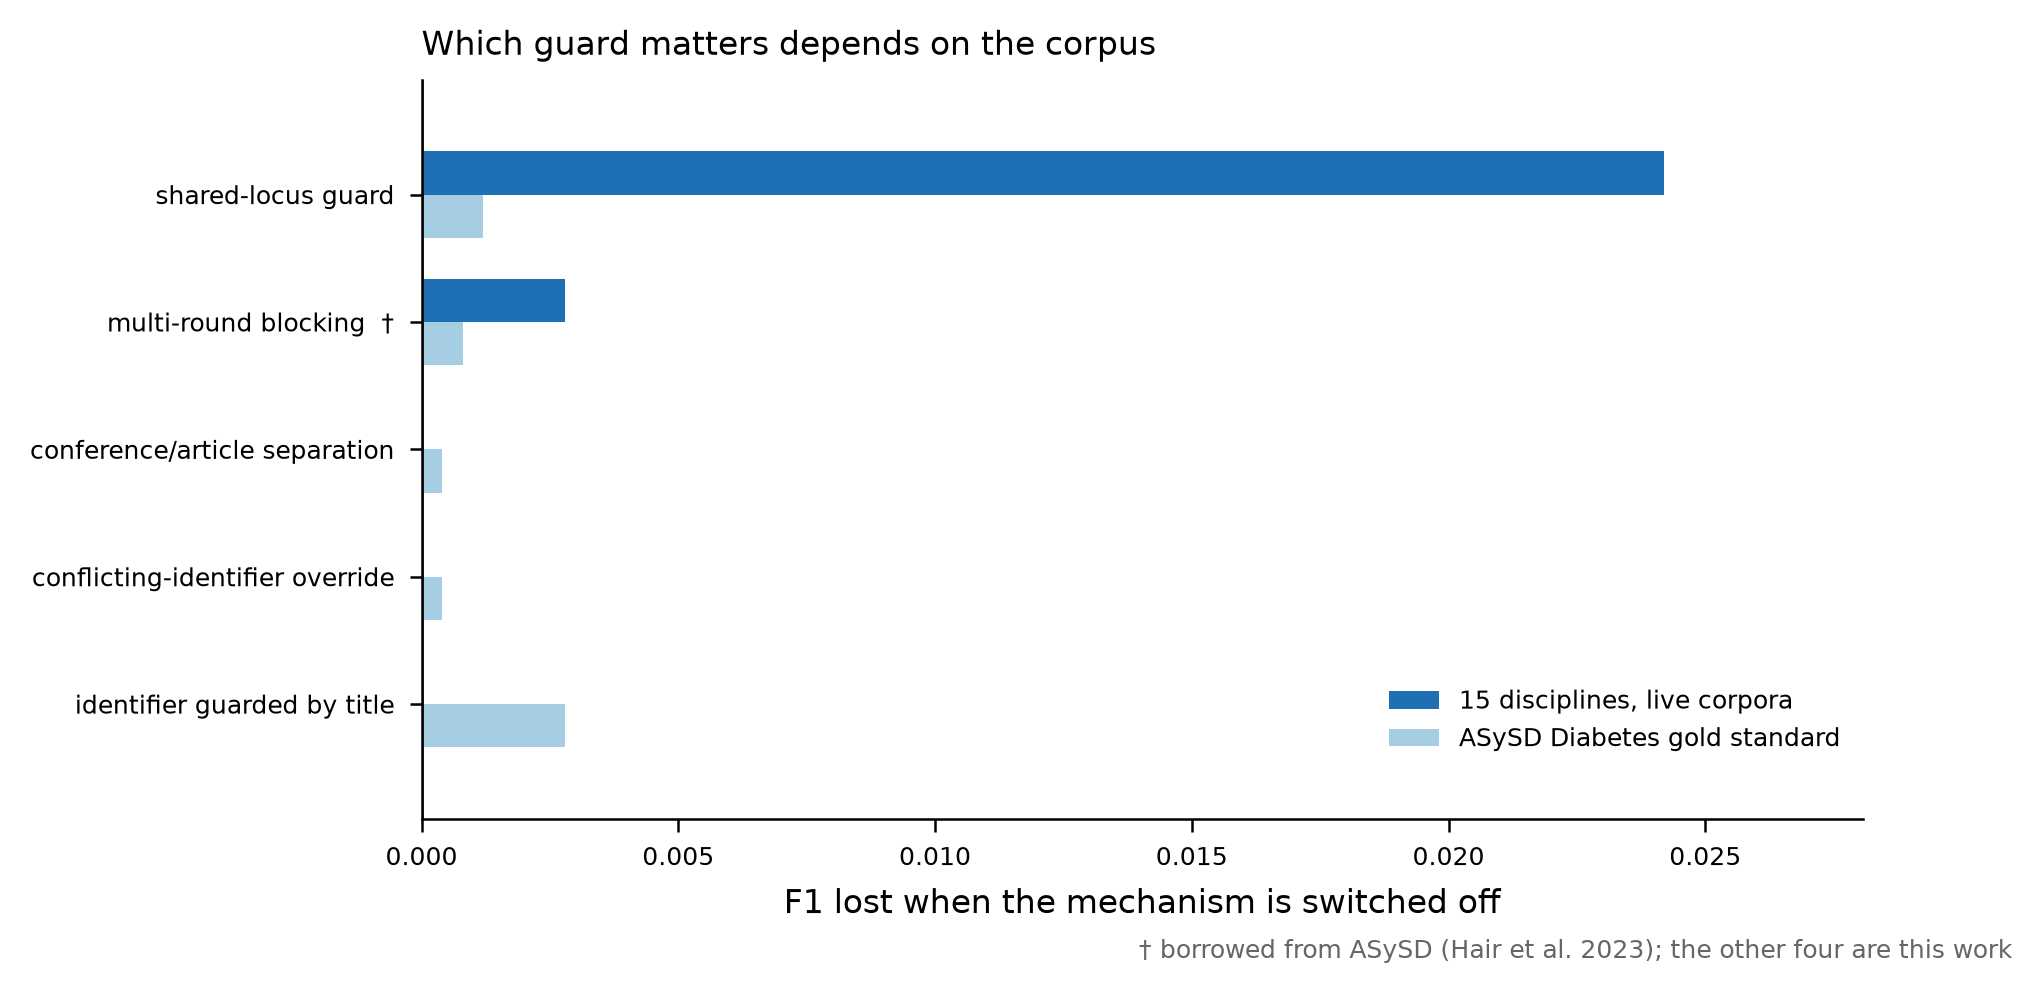
\includegraphics[width=\columnwidth]{fig_ablation.png}
\caption{Contribution of each deduplication mechanism, measured by switching
it off and rescoring. Bars are F1 lost. Multi-round blocking is borrowed from
ASySD; the other four are contributed here. The ranking inverts between the
two corpora, which is the argument for validating on more than one benchmark.}
\label{fig:ablation}
\end{figure}

\subsection{Reporting and reproducibility}

Outputs are the PRISMA 2020 flow diagram (SVG), the PRISMA-S appendix
(Markdown or .docx), a per-source metadata completeness report, an empirical
cross-source overlap matrix, the full deduplication decision log, and exports
to CSV, screening CSV, RIS and BibTeX. A harvest layer archives raw API
responses with a manifest and an order-independent checksum, so that a
reviewer can replay a search and verify that the corpus is the one the review
describes.

\subsection{The canonical output: Scopus CSV}

A review does not end at a deduplicated corpus; it continues into screening
and bibliometric analysis, and those tools read one dialect. CorpusSLR
therefore writes the merged corpus in Scopus export layout: 46 columns in the
vendor order, which is the input format that bibliometrix, VOSviewer and
EmbedSLR~\cite{embedslr2025,embedslr2026} accept. The last is the immediate
reuse path: it screens a Scopus-layout corpus by sentence embeddings, so this
library's output is its input unconverted, and bibliographic analysis of the
same file is served by packages such as TechMiner~\cite{techminer2023}.

The claim is verified by execution rather than by a column list. On a live
three-database corpus written by \texttt{to\_scopus\_csv()},
\texttt{bibliometrix::convert2df(dbsource="scopus")} under R 4.5.3 imported
166 rows with no record dropped and generated 57 bibliometrix fields;
\texttt{biblioAnalysis()} then ran on the result, and the institutional
collaboration network came out as 156 by 156 institutions. Doing this found a
defect that a column-presence check cannot see: the \texttt{Record} dataclass
had no affiliations field, so the \texttt{C1} column was always empty and the
institutional network returned an empty matrix. An
\texttt{affiliations} field was added, populated from the Web of Science
Expanded addresses node, unioned on merge and mapped to the
\texttt{Affiliations} column.

Columns with no counterpart in the harvested metadata, namely index keywords
and reference lists, are written empty rather than invented. No API in the
package returns Scopus index terms or reference lists. An empty column is
missing data the analyst can see; a fabricated affiliation or reference list
is a false finding inside someone else's co-citation network.

\subsection{Two interfaces for researchers who do not write Python}

The command \texttt{python -m corpusslr} opens a guided terminal menu built on
the standard library alone: no curses, no third-party console library, no ANSI
colour, 80 columns. It walks the user through database selection, query
construction, API keys (read with \texttt{getpass}, stored with mode 0600,
never echoed), a dry-run plan, retrieval and export. A Google Colab notebook
covers the same workflow in 26 cells for users without a local Python
installation.

\section{Illustrative examples}
\label{sec:examples}

\subsection{A minimal review in Python}

Listing~\ref{lst:api} is the library path end to end: compile a query, record
two results with their PRISMA-S provenance, deduplicate, and write the Scopus
CSV, the flow diagram and the search appendix. The two records are supplied
directly so that the example runs offline, without an API key; in a review
they would come from a client such as
\texttt{ScopusSource(api\_key=...).search(query)}. The example is kept
runnable as \texttt{paper/listing\_example.py} in the repository.

\begin{lstlisting}[language=Python,caption={A complete review in the library
API. Runs offline; the file is executed as part of preparing this
article.},label={lst:api}]
from corpusslr import (Corpus, PrismaFlow, Record, SearchQuery,
                       deduplicate, prisma_s_markdown, to_scopus_csv)

query = SearchQuery(
    blocks=[["deep learning", "convolutional neural network"],
            ["diabetic retinopathy"]],
    years=(2020, 2024), doc_types=["article"],
)
print(query.to_scopus())

corpus = Corpus()
corpus.add_records(
    [Record(title="Deep learning for diabetic retinopathy",
            doi="10.1000/ABC.123", year=2021, source="Scopus")],
    database="Scopus", platform="Elsevier",
    interface="Scopus Search API",
    query=query.to_scopus(), date_run="2026-09-07")
corpus.add_records(
    [Record(title="Deep learning for diabetic retinopathy",
            doi="https://doi.org/10.1000/abc.123", year=2021,
            source="PubMed")],
    database="PubMed", platform="NCBI", interface="E-utilities",
    query=query.to_pubmed(), date_run="2026-09-07")

result = deduplicate(corpus)
print(corpus.total_identified(), "identified ->",
      len(result.records), "unique")
print("merged by:", result.report.by_method)

to_scopus_csv(result.records, "corpus_scopus.csv")
flow = PrismaFlow.from_dedup(corpus, result)
flow.to_svg("prisma2020_flow.svg")
open("prisma_s.md", "w").write(prisma_s_markdown(corpus, result))
\end{lstlisting}

Its output shows the compiled Scopus query and the merge:

\begin{lstlisting}[caption={Output of Listing~\ref{lst:api}, as
executed.},label={lst:out}]
(TITLE-ABS-KEY("deep learning" OR "convolutional neural network"))
AND TITLE-ABS-KEY("diabetic retinopathy")
AND (PUBYEAR > 2019 AND PUBYEAR < 2025) AND (DOCTYPE(ar))
2 identified -> 1 unique
merged by: {'doi': 1}
\end{lstlisting}

The two DOIs differ in case and in the resolver prefix, which is exactly the
normalisation the identifier stage has to get right before any similarity is
computed.

The same review runs from the command line against a JSON configuration.
The \texttt{check} subcommand compiles the per-database queries and prints a
configuration checksum without issuing a single request, which is the artefact
PRISMA-S Item 8 asks for:

\begin{lstlisting}[language=bash,caption={Dry-run plan from the command-line
interface.},label={lst:cli}]
$ corpusslr check -c review.json
configuration review.json is valid
warning: no principal search system among the API databases
  (Scopus, Web of Science); Gusenbauer & Haddaway (2020)
  recommend at least one principal source
{
 "config": {
  "config_sha256": "c4240dae9b6f5a3b896accda3a350cc...",
  "corpusslr_version": "1.0.0",
  "run_at": "2026-09-08T00:43:10Z"
 },
 "databases": [
  {"database": "Crossref", "keyless": true,
   "filters": "from-pub-date:2020-01-01,type:journal-article"},
  ...
 ]
}
$ corpusslr run -c review.json
\end{lstlisting}

The registry warning in that output is the methodological guardrail of
Section~\ref{sec:description} firing at the point where the strategy can still
be changed, rather than in peer review.

\subsection{Deduplication against a published gold standard}

The guards of Section~\ref{sec:dedup} were evaluated on the labelled
\emph{Diabetes} set of Hair et
al.~\cite{hair2023} (1845 records, 1261 duplicates, 584 unique works), the
benchmark that study uses for ASySD, EndNote~\cite{bramer2016},
SRA-DM~\cite{rathbone2015} and human reviewers.
Table~\ref{tab:gold} reports the result.

\begin{table}[t]
\caption{Deduplication accuracy on the ASySD \emph{Diabetes} gold standard
($N = 1845$). Rows for the other tools are as published by Hair et
al.~\cite{hair2023} on the same data; their recall is recomputed from the
published confusion matrices, because the source tabulates precision and F1
only, and rounding in the source makes those recomputed values differ
marginally from the published ones. Data:
\texttt{validation/asysd\_metrics.csv},
\texttt{validation/na\_doi\_fix\_impact.csv}.}
\label{tab:gold}
\small
\begin{tabular}{@{}lrrrrr@{}}
\toprule
\textbf{Method} & \textbf{FP} & \textbf{FN} & \textbf{Prec.} &
\textbf{Rec.} & \textbf{F1} \\
\midrule
\textbf{CorpusSLR 1.0} & \textbf{0} & \textbf{1} & \textbf{1.0000} &
\textbf{0.9992} & \textbf{0.9996} \\
ASySD & 0 & 2 & 1.000 & 0.9984 & 0.999 \\
EndNote & 0 & 43 & 1.000 & 0.9659 & 0.983 \\
SRA-DM & 70 & 114 & 0.942 & 0.9096 & 0.926 \\
Human reviewers & 3 & 368 & 0.997 & 0.7082 & 0.828 \\
\bottomrule
\end{tabular}
\end{table}

CorpusSLR matches the published precision of the best tool on this benchmark
with no false positives and four missed duplicates against ASySD's two. The
1.7 figure is below the 0.9996 measured for version 1.3, and the difference is
informative rather than a regression: rejecting the literal \texttt{NA} as an
identifier removed 492 spurious links, and four true duplicates that had
previously been merged \emph{through} those links must now be found on title
evidence alone. The earlier figure was partly an artefact of accepting a
missing-value literal as an identifier. Two of the five error classes fixed to
reach this level were not threshold problems but normalisation defects that no
amount of tuning would have removed: percent-encoded DOIs creating a second
identity for the same work, and page fields carrying an article length rather
than a location.

\subsection{Transfer across fifteen disciplines}

Accuracy measured on one biomedical benchmark says nothing about a review in
history or logistics, and no labelled duplicate set exists for most fields.
The protocol therefore builds ground truth from the one arbiter every database
agrees on, the normalized DOI, and then \emph{deletes every identifier field},
so that deduplication must reconstruct the clusters from title, authors, year
and bibliographic coordinates alone.

Fifteen disciplines were harvested live from four databases, two queries each:
13\,809 records and 2584 judgeable pairs. Median pairwise F1 is 0.9592 and
every discipline scores above 0.85 (Table~\ref{tab:domains},
Figure~\ref{fig:domains}).

What the errors are matters more than the aggregate. Of 154 false merges, 141
are version variants of one study, such as a preprint and its published
article, two revisions of one deposit, or two editions of a chapter, and only
13 are genuine over-merges, which is 0.50\% of the judgeable pairs. Cochrane
treats versions of one study as one study, so counting them as errors measures
the arbiter rather than the implementation. Both figures are reported, in the
last two columns of Table~\ref{tab:domains}, because the choice belongs to the
review team; the median under the version-tolerant definition is 0.9806.

The variation is almost entirely in precision (0.7627 to 1.0000) rather than
recall (0.9195 to 1.0000), and it tracks publishing culture rather than
subject matter: economics scores lowest because its literature circulates as
working papers before publication. Coverage of the DOI arbiter does not
predict accuracy, since it limits how much of a corpus can be \emph{judged},
not how well it is deduplicated: computer science scores F1 0.9706 and history
0.9500.

\begin{table*}[t]
\caption{Identifier-blind deduplication across fifteen disciplines, on 13\,809
records harvested live from four databases. Pairs are judged against the
normalized DOI after every identifier field has been removed. F1$_{\text{v}}$
is the version-tolerant variant, which treats versions of one study as one
study. Totals: 13\,809 records, 2584 pairs; medians F1 0.9592 and
F1$_{\text{v}}$ 0.9806. Data: \texttt{validation/domains\_15\_final.csv}.}
\label{tab:domains}
\small
\begin{tabular}{@{}llrrrrrr@{}}
\toprule
\textbf{Discipline} & \textbf{Track} & \textbf{N} & \textbf{Pairs} &
\textbf{Prec.} & \textbf{Rec.} & \textbf{F1} & \textbf{F1$_{\text{v}}$} \\
\midrule
Economics & social & 831 & 230 & 0.7627 & 0.9783 & 0.8572 & 0.9890 \\
Logistics & social & 893 & 195 & 0.9543 & 0.9641 & 0.9592 & 0.9817 \\
Management & social & 715 & 242 & 1.0000 & 0.9587 & 0.9789 & 0.9789 \\
Marketing & social & 895 & 171 & 0.9697 & 0.9357 & 0.9524 & 0.9639 \\
Transport & social & 891 & 182 & 0.8985 & 0.9725 & 0.9340 & 0.9806 \\
Business inf. & stem & 1053 & 102 & 0.9320 & 0.9412 & 0.9366 & 0.9600 \\
Chemistry & stem & 914 & 105 & 0.9537 & 0.9810 & 0.9672 & 0.9904 \\
Computer sci. & stem & 1187 & 66 & 0.9429 & 1.0000 & 0.9706 & 0.9925 \\
Physics & stem & 1193 & 319 & 0.9750 & 0.9781 & 0.9765 & 0.9858 \\
Software eng. & stem & 617 & 149 & 0.8896 & 0.9195 & 0.9043 & 0.9547 \\
Biology & nat./hum. & 1191 & 344 & 0.9912 & 0.9855 & 0.9883 & 0.9927 \\
Geography & nat./hum. & 889 & 105 & 0.9798 & 0.9238 & 0.9510 & 0.9557 \\
History & nat./hum. & 819 & 102 & 0.9694 & 0.9314 & 0.9500 & 0.9500 \\
Political sci. & nat./hum. & 841 & 119 & 0.9914 & 0.9664 & 0.9787 & 0.9829 \\
Sociology & nat./hum. & 880 & 153 & 1.0000 & 0.9608 & 0.9800 & 0.9800 \\
\bottomrule
\end{tabular}
\end{table*}

\begin{figure}[t]
\centering
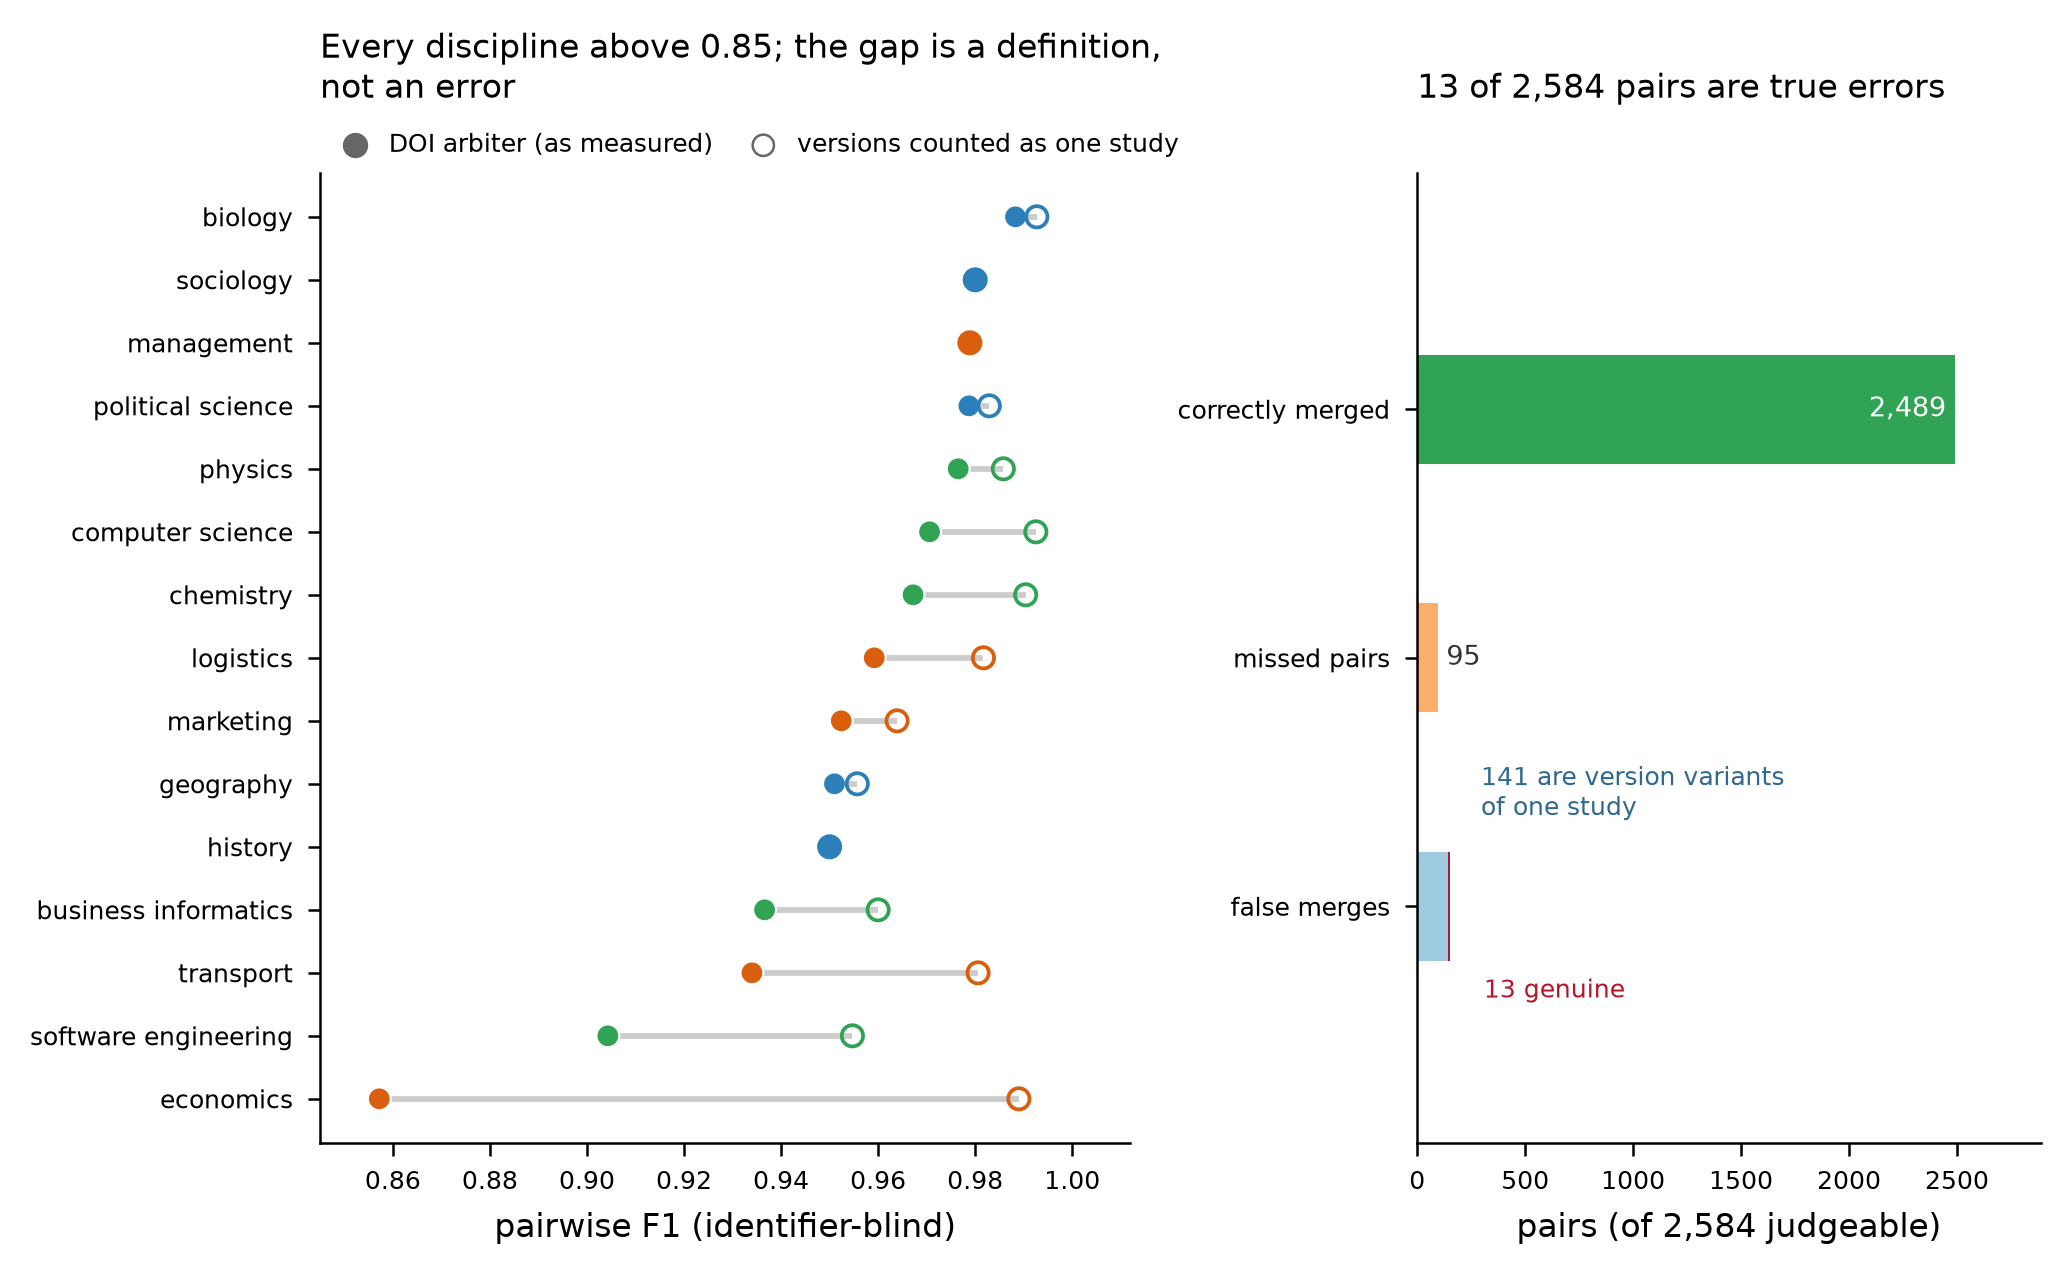
\includegraphics[width=\columnwidth]{fig_domains.png}
\caption{Deduplication across fifteen disciplines, evaluated identifier-blind
on 13\,809 live records from four databases. Left: pairwise F1 per discipline;
the filled marker scores against the DOI arbiter, the open marker treats
versions of one study as one study, and the gap between them is a definition
rather than an error. Right: composition of the 2584 judgeable pairs; of 154
false merges, 141 are version variants and 13 are genuine over-merges. Colour
marks the harvesting track, not a performance grouping.}
\label{fig:domains}
\end{figure}

\subsection{Scale and live behaviour}

On synthetic corpora with 20\% planted cross-source duplicates,
deduplication processes 60\,000 records in 25.3 s at 310 MB peak
(422.3 microseconds per record), while a pathological corpus in which every
title shares a stock opening takes 9.6 s and 109 MB. Unit cost rises from
260.3 to 422.3 microseconds per record over a tenfold increase in corpus size,
so scaling is close to linear but not exactly so. The cost is dominated by
title comparison, and memoising the normalized title is what makes it
tractable.

Running the retrieval layer against the live services exposed three defects
that offline tests cannot reach: the Scopus client defaulted to the leaner
response view, which returns one author and no abstract at all, making
title and abstract screening impossible; the preprint client had no scan
budget, so a selective query over a multi-year window became an hours-long
full-archive crawl; and the Web of Science client addressed the Starter API
while an entitled subscription serves Expanded. On a live Web of Science
Expanded query, the client returned an abstract on 100 of 100 records where
Starter returns none.

\section{Impact}
\label{sec:impact}

The measurements of Section~\ref{sec:examples} support three claims of impact.
The immediate one is on compliance work that currently consumes reviewer
and author time. The PRISMA-S appendix is generated from recorded provenance,
so the database, platform and interface triple, the executed strategy, the
dates and the per-database counts cannot drift from what was actually run.
Deduplication performs at the level of the best published tool while producing
an auditable decision log, which converts ``duplicates were removed in EndNote''
into a reportable and checkable method.

The second impact is methodological guardrails. The registry makes the
principal and supplementary distinction operational rather than advisory: a
corpus built only from supplementary systems raises a critical warning at the
point where it can still be fixed. To our knowledge this classification has
not been automated in a review-support library before.

The third is reproducibility, in the sense of the FAIR
principles~\cite{wilkinson2016}, at two levels. A harvest archive with a manifest
and an order-independent checksum lets a reviewer replay a search and confirm
the corpus. And a whole review, from search through parsing, deduplication,
diagram and appendix, runs from one JSON configuration through the
command-line interface, so that the reported method is the method that
executed. The dry-run mode of Listing~\ref{lst:cli} compiles the per-database
queries with a configuration checksum before any request is made.

Because the canonical export is the Scopus layout, the corpus continues
directly into the established bibliometric toolchain rather than terminating
in a bespoke format, which is what makes the package usable as one stage of an
existing workflow instead of a replacement for it.

\section{Conclusions}
\label{sec:conclusions}

CorpusSLR covers the span from a structured query to a PRISMA-compliant,
deduplicated and auditable corpus, which is the chain
Section~\ref{sec:motivation} identifies as unautomated, and it delivers the
reporting artefacts of Section~\ref{sec:impact} from recorded provenance.
Deduplication is validated against a
published gold standard, where it reaches F1 0.9996, and across fifteen
disciplines under an identifier-blind protocol, where the median pairwise F1
is 0.9592 and the 154 false merges resolve into 141 version variants and 13
genuine over-merges.

The limitations are stated plainly. The cross-disciplinary arms are small in
pairs judged per discipline, between 66 and 344, and no confidence intervals
are reported. Citation-based strategies such as snowballing~\cite{wohlin2014} are outside
its scope. Thesaurus expansion, such as MeSH or Emtree, is not performed,
so a librarian-designed strategy still outperforms a compiled one in
biomedical databases. The measured accuracy across disciplines depends on DOI
coverage in the harvested sample, which bounds how much of a corpus can be
judged at all. And the ablation shows that the ranking of the deduplication
guards inverts between the two benchmarks, so the shipped defaults are a
compromise rather than an optimum for any single field.

\section*{Acknowledgements}

The evaluation rests on the labelled deduplication benchmark published by
the ASySD authors, whose decision to release it openly is what made an
external comparison possible. Clarivate granted the Web of Science
Expanded API entitlement used to verify that client against the live
service.

\section*{Declaration of competing interest}

The author declares no competing interests.

\section*{Data availability}

All data underlying the results are public. The software, the evaluation
scripts and the measurement tables are in the repository given in C2. The
validation data are additionally packaged for review as
\texttt{corpusslr\_validation\_data.zip}, whose manifest maps each file to the
table or figure it supports. One file is third-party: the ASySD \emph{Diabetes}
gold standard, redistributed unmodified from
\texttt{github.com/camaradesuk/ASySD} under that project's GPL-3.0 licence,
with provenance, pinned commit and checksum recorded in
\texttt{validation/THIRD\_PARTY\_DATA.md}. The corpora harvested for the
cross-disciplinary study are archived as compressed record dumps, so every
number reported here recomputes without network access.

\bibliographystyle{elsarticle-num}
\bibliography{references}

\end{document}
